

\input{header}

% *** Do not adjust lengths that control margins, column widths, etc. ***
% *** Do not use packages that alter fonts (such as pslatex).         ***
% There should be no need to do such things with IEEEtran.cls V1.6 and later.
% (Unless specifically asked to do so by the journal or conference you plan
% to submit to, of course. )


% correct bad hyphenation in this file
% correct bad hyphenation here
\hyphenation{
  Be-schleu-ni-gungs-sen-sor
  Durch-sicht-bril-le
  Drift-kor-rek-tur
  Erd-mag-net-feld
  Fahr-zeug-e-lek-tro-nik
  Iner-tial-sy-stem
  Ma-g-ne-to-me-ter
  net-works
  op-tical
  semi-conduc-tor
  Ver-ar-bei-tungs-pipe-line
  Wheat-stone-sche
}



\begin{document}


\begin{acronym}

  \acro{AR}{Augmented Reality}
  \acro{IMU}{Inertial Measurement Unit}
  \acro{INS}{Inertiales Navigationssystem}
  
\end{acronym}


%
% paper title
% can use linebreaks \\ within to get better formatting as desired
\title{Projektpraktikum Kognitive Automobile:\\
Virtuelles Testen}
%
%
% author names and IEEE memberships
% note positions of commas and nonbreaking spaces ( ~ ) LaTeX will not break
% a structure at a ~ so this keeps an author's name from being broken across
% two lines.
% use \thanks{} to gain access to the first footnote area
% a separate \thanks must be used for each paragraph as LaTeX2e's \thanks
% was not built to handle multiple paragraphs
%
%
%\IEEEcompsocitemizethanks is a special \thanks that produces the bulleted
% lists the Computer Society journals use for "first footnote" author
% affiliations. Use \IEEEcompsocthanksitem which works much like \item
% for each affiliation group. When not in compsoc mode,
% \IEEEcompsocitemizethanks becomes like \thanks and
% \IEEEcompsocthanksitem becomes a line break with idention. This
% facilitates dual compilation, although admittedly the differences in the
% desired content of \author between the different types of papers makes a
% one-size-fits-all approach a daunting prospect. For instance, compsoc 
% journal papers have the author affiliations above the "Manuscript
% received ..."  text while in non-compsoc journals this is reversed. Sigh.

% Alphabetisch nach Nachnamen sortiert:
\author{
{\normalsize
Maximilian Baritz,
Johannes Bittner,
Matthias Eisenmann,
Francesco Gerardi,
Daniel Hammann,
Tobias Roth,
Tam Nguyen,
Dmitrij Sarancin,
Christian Vogt,
Ecaterina X.
 \\
Betreuer: \diplinf Ralf Kohlhaas, \msc Marc Rene Zofka
}

%\IEEEcompsocitemizethanks{\IEEEcompsocthanksitem M. Shell is with the Department
%of Electrical and Computer Engineering, Georgia Institute of Technology, Atlanta,
%GA, 30332.\protect\\
%% note need leading \protect in front of \\ to get a newline within \thanks as
%% \\ is fragile and will error, could use \hfil\break instead.
%E-mail: see http://www.michaelshell.org/contact.html
%\IEEEcompsocthanksitem J. Doe and J. Doe are with Anonymous University.}% <-this % stops a space
%\thanks{Manuscript received April 19, 2005; revised January 11, 2007.}
}

% note the % following the last \IEEEmembership and also \thanks - 
% these prevent an unwanted space from occurring between the last author name
% and the end of the author line. i.e., if you had this:
% 
% \author{....lastname \thanks{...} \thanks{...} }
%                     ^------------^------------^----Do not want these spaces!
%
% a space would be appended to the last name and could cause every name on that
% line to be shifted left slightly. This is one of those "LaTeX things". For
% instance, "\textbf{A} \textbf{B}" will typeset as "A B" not "AB". To get
% "AB" then you have to do: "\textbf{A}\textbf{B}"
% \thanks is no different in this regard, so shield the last } of each \thanks
% that ends a line with a % and do not let a space in before the next \thanks.
% Spaces after \IEEEmembership other than the last one are OK (and needed) as
% you are supposed to have spaces between the names. For what it is worth,
% this is a minor point as most people would not even notice if the said evil
% space somehow managed to creep in.



% The paper headers
\markboth{Projektpraktikum: Kognitive Automobile WS2013/2014}%
{Shell \MakeLowercase{\textit{et al.}}: Bare Advanced Demo of IEEEtran.cls for Journals}
% The only time the second header will appear is for the odd numbered pages
% after the title page when using the twoside option.
% 
% *** Note that you probably will NOT want to include the author's ***
% *** name in the headers of peer review papers.                   ***
% You can use \ifCLASSOPTIONpeerreview for conditional compilation here if
% you desire.



% The publisher's ID mark at the bottom of the page is less important with
% Computer Society journal papers as those publications place the marks
% outside of the main text columns and, therefore, unlike regular IEEE
% journals, the available text space is not reduced by their presence.
% If you want to put a publisher's ID mark on the page you can do it like
% this:
%\IEEEpubid{0000--0000/00\$00.00~\copyright~2007 IEEE}
% or like this to get the Computer Society new two part style.
%\IEEEpubid{\makebox[\columnwidth]{\hfill 0000--0000/00/\$00.00~\copyright~2007 IEEE}%
%\hspace{\columnsep}\makebox[\columnwidth]{Published by the IEEE Computer Society\hfill}}
% Remember, if you use this you must call \IEEEpubidadjcol in the second
% column for its text to clear the IEEEpubid mark (Computer Society jorunal
% papers don't need this extra clearance.)



% use for special paper notices
%\IEEEspecialpapernotice{(Invited Paper)}



% for Computer Society papers, we must declare the abstract and index terms
% PRIOR to the title within the \IEEEcompsoctitleabstractindextext IEEEtran
% command as these need to go into the title area created by \maketitle.
\IEEEcompsoctitleabstractindextext{%

\begin{abstract}
Diese Ausarbeitung fasst die Ergebnisse des Projektpraktikums Kognitive Automobile zusammen, welches sich im Wintersemester 2013/2014 mit dem Thema \emph{virtuelles Testen} im Bereich des autonomen und semi-autonomen Fahrens beschäftigt.

Die Aspekte ``driverless and self-driving'' gewinnen in der heutigen Automobil- und Robotik-Industrie immer mehr an Bedeutung.
Dabei sind effiziente und kostengünstige Testmethoden für diese Themengebiete wichtiger denn je.
Diese Ausarbeitung handelt von der Konzipierung und Realisierung einer virtuellen Test- und Simulationsumgebungen, welche die Möglichkeit bieten soll Fahrsituationen auch ohne realen Verkehr nachzubilden.

Es sollen dafür Szenarien für Testfahrten erstellt werden, die durch Objekteinblendung mittels einer Augmented-Reality-Brille die Grundlage der Testumgebung bilden.
Dieser Ansatz stellt eine effiziente Alternative zum realen Testen dar und ermöglicht es Testszenarien beliebig oft und unfallfrei reproduzieren zu können.
Bevor es soweit ist, muss die Brille korrekt für den Einsatz im Versuchsträger installiert werden.
Dies wird über das sogenannte \textit{Headtracking} umgesetzt, welches eine Orientierung der Kopfposition des Fahrers liefert. 
Diese wird dann als Grundlage für die anschließende Objekteinblendung, auch im bewegenden Fahrzeug, eingesetzt.
\end{abstract}


% IEEEtran.cls defaults to using nonbold math in the Abstract.
% This preserves the distinction between vectors and scalars. However,
% if the journal you are submitting to favors bold math in the abstract,
% then you can use LaTeX's standard command \boldmath at the very start
% of the abstract to achieve this. Many IEEE journals frown on math
% in the abstract anyway. In particular, the Computer Society does
% not want either math or citations to appear in the abstract.

% Note that keywords are not normally used for peerreview papers.
\begin{IEEEkeywords}
Autonomous Driving, Augmented Reality, Virtual Testing, Headtracking, Vuzix Glasses, Filtering, Sensors, Sensor Fusion, IMU, Magnetometer, Marker Tracking, Loosely Coupled System
\end{IEEEkeywords}}


% make the title area
\maketitle


% To allow for easy dual compilation without having to reenter the
% abstract/keywords data, the \IEEEcompsoctitleabstractindextext text will
% not be used in maketitle, but will appear (i.e., to be "transported")
% here as \IEEEdisplaynotcompsoctitleabstractindextext when compsoc mode
% is not selected <OR> if conference mode is selected - because compsoc
% conference papers position the abstract like regular (non-compsoc)
% papers do!
\IEEEdisplaynotcompsoctitleabstractindextext
% \IEEEdisplaynotcompsoctitleabstractindextext has no effect when using
% compsoc under a non-conference mode.


% For peer review papers, you can put extra information on the cover
% page as needed:
% \ifCLASSOPTIONpeerreview
% \begin{center} \bfseries EDICS Category: 3-BBND \end{center}
% \fi
%
% For peerreview papers, this IEEEtran command inserts a page break and
% creates the second title. It will be ignored for other modes.
\IEEEpeerreviewmaketitle


% generelle todo's
\todo[inline]{PDF-Infos anpassen}
\todo[inline]{Alle Bilder mit Quellen?!}
\todo[inline]{Nach '??' scannen}
\todo[inline]{Nach Overflows scannen (im draft Modus bauen)}


% Inhalt


\section{Einführung}
\label{einleitung_sec}

Thema des Projektpraktikums \emph{Kognitive Automobile} ist es, eine virtuelle Test- und Simulationsumgebung für reale Erprobungsfahrten in einem autonomen Fahrzeug zu erzeugen.
Dies geschieht unter Zuhilfenahme einer 3D-Augmented-Reality-Brille mit Headtracker, welche in den \ac{FZI}-Versuchträger CoCar integriert wird.


\subsection{Motivation}
\label{einleitung_motivation_subsec}


Neuentwicklungen im Bereich des autonomen Fahrens müssen ausgiebig getestet werden, bevor sie in Fahrzeugen Anwendung finden können.
Simulationen sind zum Testen ein geeignetes Mittel, sie geraten jedoch häufig an ihre Grenzen.
Daher ist es in der Entwicklung von autonomen Fahrfunktionen unerlässlich, diese auch im realen Fahrbetrieb zu testen.

In bestimmten Szenarien (beispielsweise eine Notbremsung aufgrund eines Fußgängers oder autonomes Einparken im Parkhaus) ist Testen in der Realität allerdings gefährlich.
Das Risiko, einen Probanden zu verletzen bzw. mit der teuren Versuchsplattform gegen die Parkhauswand zu stoßen, kann nicht eingegangen werden.

Für solche Fälle ist eine hybride Umgebung, bestehend aus realer Versuchsplattform und simulierter Umgebung, ein möglicher Ansatz.
Der Sicherheitsfahrer bekommt dazu simulierte Hindernisse in der \ac{AR}-Brille eingeblendet und kann die Reaktion des Autos in der Realität überwachen.

Die Anwendung einer solchen \ac{AR}-Brille kann ebenso zur Einblendung von weiteren Daten wie beispielsweise aktuellen Manöver-, Navigations- oder Entertainment-Informationen verwendet werden.

%Was ist damit?  --> siehe commit-comment 77d294a54
%Im Kontext Kognitiver Automobile hat eine Kalibrierte 3D Sicht ebenfalls eine große Bedeutung: Hierbei gibt es zwei große Anwendungsgebiete, einerseits können hiermit neue Geräte oder Anzeigen Simuliert werden, andererseits kann hiermit aber auch eine Simulierte Realität dem Sicherheitsfahrer angezeigt werden. So wird z.B. ein Auffahrbremsen simuliert, so kann dem Fahrer das Simulierte Auto angeziegt werden. Oder wird in eine simulierte Parkbuch eingeparkt, so kann diese vom Sicherheitsfahrer durhc die Brille beurteilt werden.


\subsection{Aufgabenstellung}
\label{einleitung_aufgabenstellung_subsec}


In diesem Projektpraktikum soll ein wie in Absatz \ref{einleitung_motivation_subsec} beschriebenes hybrides System entwickelt werden.

Die wesentlichen Komponenten für eine solche \ac{AR}-Umgebung sind:
\begin{itemize}
  \item Headtracking zur Bestimmung der Kopforientierung
  \item Augenbezogene Einblendung von Objekten
\end{itemize}

Für die Bestimmung der Kopforientierung soll primär die Inertialsensorik der \ac{AR}-Brille verwendet werden.
Die Kompensation der Eigenbewegung des Fahrzeugs ist unter Zuhilfenahme weiterer Sensorik zu bewältigen.
Zur Verfügung stehen die Inertialsensorik des Autos, die im Auto verbaute Kinect-Sensorleiste sowie die direkt auf der \ac{AR}-Brille montierte Kamera.

Des Weiteren soll untersucht werden, wie eine augenbezogene Einblendung von Objekten in das Sichtfeld des Fahrers mittels der \ac{AR}-Brille ermöglicht werden kann. Dafür ist zum einen eine Auge-Display-Kalibrierung vorzunehmen.
Zum anderen sollen anzuzeigende Objekte für eine 3D-Einblendung aufbereitet werden (Stereoskopisches 3D).

\subsection{Hard- und Software}
\label{einleitung_hardware_subsec}

Für die beschriebene Aufgabenstellung steht als Hardware eine \ac{AR}-Brille des Herstellers \emph{Vuzix} vom Typ \emph{Star 1200} zur Verfügung, s. Abb. \ref{fig:vuzix_star_1200}.
Diese besitzt folgende Merkmale:
\begin{itemize}
  \item 2 vor den Augen angebrachte transparente Displays (Blickwinkel ca. $30^\circ$)
  \item 1 feste Kamera (Logitech Webcam)
  \item \ac{IMU} (\emph{Wrap Tracker 6TC}), bestehend aus 2 Gyroskopen, Beschleunigungssensor sowie Magnetometer
\end{itemize}

\begin{figure}[h]
  \centering
  %\missingfigure{Vuzix}
  \includegraphics[width=0.4\textwidth]{vuzix}
  \caption{\ac{AR}-Brille \emph{Vuzix Star 1200}\ \cite{vuzix}}
  \label{fig:vuzix_star_1200}
\end{figure}

Für die Programmierung stehen die \ac{ICL}-Softwareumgebung des \ac{FZI}, sowie das \ac{ROS}-Framework \cite{ros} zur Verfügung.



\section{Headtracking}

Ziel des Headtrackings ist es, die Kopforientierung des Fahrers --auch bei bewegtem Fahrzeug--
%\todo{``fahrendem'' statt ``bewegendem''?}
% -> ich würde bei bewegt bleiben: es ist ja denkbar, dass das Auto nicht selber "fährt", aber trotzdem "bewegt" wird, beispielsweise auf einer Fähre oder so
sowohl relativ zum Fahrzeug als auch in Weltkoordinaten anzugeben. Unter Orientierung wird hier die Drehung entlang der X (\emph{Roll}), Y (\emph{Pitch}) und Z-Achse (\emph{Yaw}) verstanden:
\acs{RPY}.

Dazu wird die Inertialsensorik der \ac{AR}-Brille, bestehend aus zwei Gyroskopen, Beschleunigungssensor und Magnetometer, ausgewertet (Abs. \ref{headtracking_imu_subsec}).
Diese Daten werden mit einem geeigneten Filter-Algorithmus fusioniert (Abs. \ref{headtracking_fusion_subsec}).
Die Kompensation der Eigenbewegung des Fahrzeugs wird in Abs. \ref{headtracking_marker_subsec} behandelt.


\subsection{Inertialsensoren}
\label{headtracking_imu_subsec}


\subsubsection{Gyroskop}
\label{headtracking_imu_gyro_subsubsec}

Das in der Brille enthaltene Gyroskop misst Winkelgeschwindigkeiten in
$\omega = [{Grad \over Sekunde}]$ bei Drehungen um die X, Y und Z-Achse. Durch
die Integration der Winkelgeschwindigkeiten über die Zeit kann die
Orientierung der Brille bestimmt werden.  

Die \ac{IMU} der Brille enthält zwei
Gyroskope, ein \emph{High Bandwidth} Gyrosokp sowie ein
\emph{Low Bandwidth} Gyroskop. Die Gyroskope unterscheiden sich
hinsichtlich der Genauigkeit und des Wertebereiches. Das \ac{HBW}-Gyroskop
hat einen größeren Wertebereich, jedoch die geringere
Genauigkeit.

Die Rohdaten des Sensors enthalten einen konstanten Versatz, so dass bei
stationärer Brille eine Geschwindigkeit $\omega \neq 0$ gemessen wird. Dieser
Versatz wird \emph{Bias} genannt, und muss in einem stationären
Kalibriervorgang ermittelt werden. Während des Kalibriervorganges wird
der Bias gemittelt, dieser wird nach Beendigung des Kalibriervorganges von den
Rohdaten abgezogen. Abb. \ref{fig:gyro_bias} zeigt die Daten vor und nach der
Bias-Korrektur.

\begin{figure}[h]
   \centering
   \includegraphics[width=0.45\textwidth]{stationary_calibration_before_after}
   \caption{Korrektur des Gyroskop-Bias}
   \label{fig:gyro_bias}
\end{figure}

Desweiteren unterliegen die Sensordaten einem Rauschen. Daher wird als
nächster Schritt ein Tiefpassfilter verwendet, um dieses Rauschen zu
reduzieren. In unserem Fall hat sich ein Mittelwertfilter mit einer 
Fenstergröße von 5 als praktikabel erwiesen. Je höher die Fenstergröße gewählt wird,
desto stärker werden die Rohdaten geglättet, damit steigt jedoch auch
die Verzögerung der Daten. Abb. \ref{fig:lowpass-delay} zeigt den Effekt des Tiefpassfilters.

\begin{figure}[h]
   \centering
   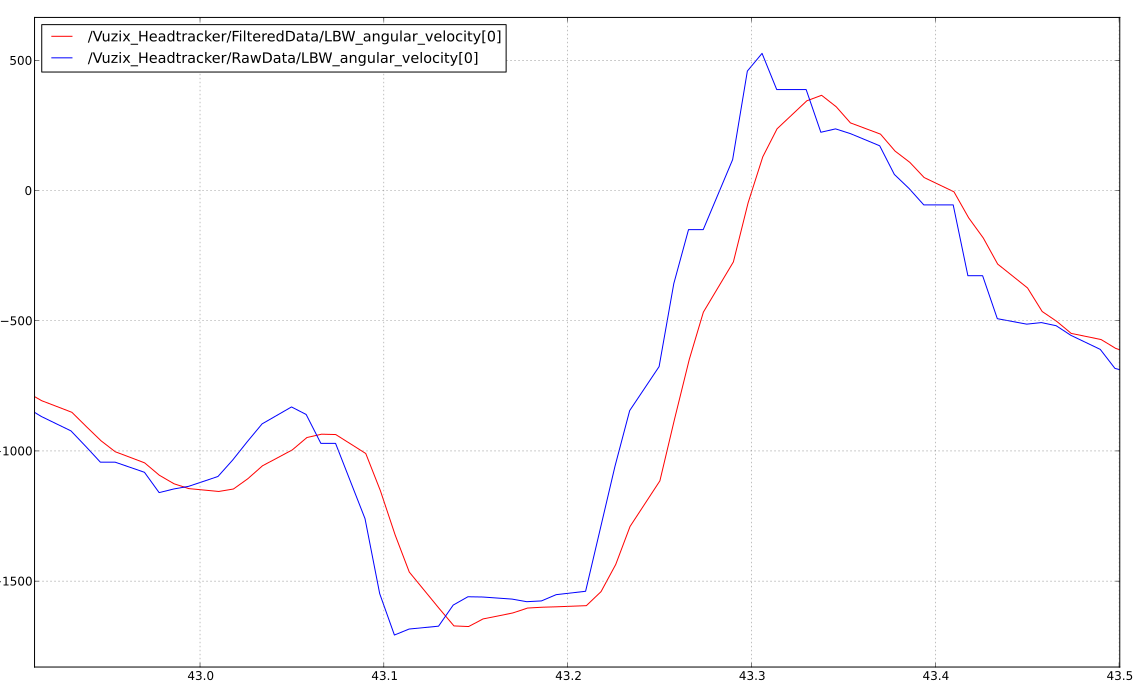
\includegraphics[width=0.45\textwidth]{FilteringDelay}
   \caption{Auswirkung des Tiefpassfilters: Ungefilterte Daten (blau) vs. gefilterte Daten (rot)}
   \label{fig:lowpass-delay}
\end{figure}

Die Wertebereiche der Gyroskope sind
in Tab. \ref{tab:ranges-gyros} aufgeführt. Beide Gyroskope liefern
einen 12-Bit-Datenwert. Somit stellt ein Zählwert des \ac{LBW}-Gyroskops eine
kleinere Veränderung dar als beim \ac{HBW}-Gyroskop.
Dies bedeutet, dass das \ac{LBW}-Gyroskop eine höhere Genauigkeit besitzt.

\begin{table}[ht]
  \centering
  \begin{tabular}{ | c | c | c | }
    \hline
    & Min. & Max. \\ \hline
    \ac{LBW} & -420   & 420   \\ \hline
    \ac{HBW} & -1680   & 1680   \\
    \hline
  \end{tabular}
  \caption{Gyroskop-Wertebereiche in $[{\degree \over s}]$}
  \label{tab:ranges-gyros}
\end{table}


Zur Fusionierung des \ac{HBW}- und \ac{LBW}-Gyroskops kommt ein einfaches Schwellwertverfahren zum Einsatz. 
Im Wertebereich, welcher von beiden Gyroskopen abgedeckt wird, werden
die Sensordaten gemittelt. Wird der Wertebereich des \ac{LBW}-Gyroskops
überschritten, wird lediglich der Wert des \ac{HBW}-Gyroskops
zurückgeliefert.

\begin{equation}
    G = \left\{
    \begin{array}{ll}
        \frac{G_{HBW} + G_{LBW}}{2}, & G_{LBW} < G_{LBW_{max}}  \\
        G_{HBW}, & G_{LBW} = G_{LBW_{max}}
    \end{array}\right. \\
\end{equation}

Aus den gefilterten Sensordaten wird daraufhin durch Integration über
die Zeit die Orientierung berechnet. Hierzu wird die Orientierung in einem Quaternion gespeichert, welches nach jeder Sensor-Abtastung aktualisiert wird. Hierbei ist $dt$ die Abtastrate der Gyroskop-Sensoren\todo{beträgt 200Hz(?)}.

\begin{equation}
    \Delta q = quaternion({\omega_x \over dt}, {\omega_y \over dt}, {\omega_z \over dt}) \\
\end{equation}

\begin{equation}
    q = q * \Delta q
\end{equation}

Die durch das Gyroskop berechnete Orientierung reagiert schnell auf
Änderungen. Durch die Integration entsteht in jedem Integrationsschritt jedoch ein Fehler, welcher sich summiert. Dieser Fehler wird als \emph{Drift} bezeichnet. In den folgenden Abschnitten wird beschrieben wie Beschleunigungssensor und Magnetometer verwendet werden können, um diesen Fehler zu kompensieren.

% TR: Schöner Abschnitt  :-)


\subsubsection{Beschleunigungssensor}


Der Beschleunigungssensor misst die Gravitation entlang der X, Y und Z-Achse, im Folgenden als $acc_x$, $acc_y$ und $acc_z$ bezeichnet.
\todo[inline]{TR: Das ist meiner Meinung nach falsch, es wird die Beschleunigung gemessen! Gravitation ist eine Untermenge davon. Was der Sensor misst, ist: Gravitation + Beschleunigung beispielsweise durch Kopf/Auto-Bewegung!}
Anhand dieses Gravitationsvektors kann die Orientierung der Brille bezüglich der horizontalen Ebene bestimmt werden\todo{s. vorigen Kommentar}.

Zur Verwendung des Beschleunigungssensors wird zunächst wie auch beim
Gyroskop ein Tiefpassfilter angewendet, um das Rauschen der Rohdaten zu
reduzieren.
Dabei wird ein Mittelwertfilter eingesetzt.
Als Fenstergröße wird die gleiche wie beim Gyroskop gewählt, da ein ungleicher Wert zu Fehlern bei der späteren Fusion
führen würde. 

% XXX: die umrechung auf m/s2 hab ich mal rausgelassen, die ist ja glaub ich auch garnicht so wichtig und verwirrt den leser nur

Die Orientierung in Roll und Pitch kann direkt aus den Winkeln des Gravitationsvektors berechnet werden.

\begin{equation}
    roll = atan2(acc_y, acc_z)
\end{equation}

\begin{equation}
    pitch = -atan2(acc_x, \sqrt{ {acc_y}^2 + {acc_z}^2 })
\end{equation}

Die so bestimmten Roll und Pitch Werte sind frei von Drift, und können als Stützwerte für die aus den Gyroskopdaten berechneten Orientierungswerte verwendet werden.
Jedoch ist zu beachten, dass der Beschleunigungssensor nicht zuverlässig zur Berechnung des Yaw-Winkels verwendet werden kann.
Dies liegt darin begründet, dass sich die Sensordaten des Beschleunigungssensors nicht ändern, wenn sich der Sensor parallel zur Erdoberfläche befindet und um den Yaw-Winkel gedreht wird.


%  roll = atan2(acc_data[1], acc_data[2]);
%  pitch = -atan2(acc_data[0], sqrt(acc_data[1]*acc_data[1] + acc_data[2]*acc_data[2]));


\subsubsection{Magnetometer}
\label{headtracking_magnetometer_subsubsec}
Das Magnetometer wird im Rahmen des Praktikums zur Stützung des Yaw-Winkels (Drehung um die Z-Achse des Brillenkoordinatensystem) genutzt.\\
Das verbaute Magnetometer misst in drei Achsen nach dem Funktionsprinzip der Wheatstoneschen Messbrücke \cite{renaudin2010complete} das Erdmagnetfeld.
Dieses Messverfahren führt zum einen zu einer kleinen und kostengünstigen Bauweise.
Zum anderen entstehen aber Messungenauigkeiten, die im Rahmen der Sensorkalibrierung beachtet und ausgeglichen werden müssen.

\begin{figure}
   \centering
   \includegraphics[width=0.4\textwidth]{earth-magnetic-field}
   \caption[mag_world]{Schematische Darstellung des Erdmagnetfelds \cite{mag_world_source}.}
   \label{fig:mag_world}
\end{figure}

\begin{figure}
   \centering
   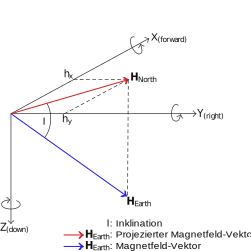
\includegraphics[width=0.4\textwidth]{magnetometer-yaw-calculation}
   \caption[mag_mapping]{Berechungsgrundlage des Magnetfeldvektors}
   \label{fig:mag_mapping}
\end{figure}

Gemessen werden die Magnetfeldlinien der Erde, welche in Abbildung \ref{fig:mag_world} dargestellt sind.
Diese sind abhängig von der aktuellen Position auf der Erdoberfläche\footnote{Tatsächlich verändert sich das Erdmagnetfeld auch über die Zeit hinweg.
Diese Änderung kann aber im Rahmen des Praktikums vernachlässigt werden, da es sich um eine sehr kleine Änderung handelt (z. Bsp. für den Praktikumsort Karlsruhe ca. $1^\circ 46$'~$7.8$ arcmin/Jahr im Deklinationswinkel).}.
Sobald das Erdmagnetfeld nicht am Äquator gemessen wird, sondern im Falle unseres Praktikums bei etwa $49^\circ$ geographischer Breite muss der Inklinationswinkel bei der Messung mit beachtet werden, welcher in Abbildung \ref{fig:mag_mapping} mit I beschrieben wird.
Diese Abbildung auf die XY-Ebene wird durch folgende Formel bewerkstelligt:

\begin{equation}
    \varphi = atan2(h_y,h_x)
\end{equation}

Dabei sind $h_x$ und $h_y$ die Anteile des Magnetfeldvektors $H_{Earth}$ in X sowie Y Richtung.

Der gemessene 3D-Magnetfeldvektor ist zunächst unkalibriert und einheitenlos.
Daher ist zuerst eine Kalibrierung der gemessenen Werte notwendig um sie weiterverarbeiten zu können. 
Diese Kalibrierung hat zum Ziel einen Kanal-spezifischen Bias auszugleichen. 
Dieser entsteht durch die bereits angesprochenen Messungenauigkeiten des Sensors sowie durch sogenannte \textit{Hard Iron}-Störeffekte, welche durch eigenständige Magnetquellen induziert werden.
Beispiele für diese Störeffekte, sowie die letztlich kalibrierten Daten sind in Abbildung \ref{fig:mag_kugel_plots} als Kugelplots dargestellt.

\begin{figure}[ht]
\centering
\subfigure[Unkalibrierte Magnetometerdaten mit Hard Iron Störeinflüssen]{
    \includegraphics[width=0.5\textwidth]{uncalibrated}
    \label{fig:subfig1}
}
\subfigure[Kalibrierte Magnetometerdaten]{
    \includegraphics[width=0.5\textwidth]{calibrated}
    \label{fig:subfig2}
}

\caption[]{2D-Sichten auf Kugel aus Magnetometerdaten}
\label{fig:mag_kugel_plots}
\end{figure}

Im Gegensatz zu den bisher vorgestellten Sensoren wird die Kalibrierung des Magnetometers durch Bewegung durchgeführt.
Ziel ist es, die Wertebereiche in allen drei Achsen zu erfassen.
Dafür wird die Brille in allen Achsen um mindestens $360^\circ$ gedreht, um die minimalen und maximalen Werte zu registrieren. 
Des weiteren wurden die Daten noch durch einen Tiefpassfilter geglättet sowie auf einen Wertebereich von $[-1,1]$ abgebildet.
 Der Tiefpassfilter wurde wie in Abs. \ref{headtracking_imu_gyro_subsubsec} bereits beschrieben durchgeführt. 
Die Anwendung der Kalibrierung und Normierung wird durch nachfolgende Formel bewerkstelligt:
\begin{equation}
    m_{norm} = \frac{m_{raw}- \frac{m_{\delta}}{2}}{2~m_{\delta}},~mit ~m_{\delta} = m_{max} - m_{min}
\end{equation}
Dabei bezeichnet $m_{norm}$ einen normierten Magnetfeldvektorkanal, $m_{raw}$ die Rohdaten des jeweiligen Kanals und $m_{\lbrace max, min\rbrace}$ den gemessenen Maximal- bzw. Minimalwert.
Ursprünglich war die Verwendung des Magentometers zur Stützung des Yaw-Winkels fraglich, da der Einsatz im Versuchsträger CoCar viele magnetische Störquellen in Form der vorhandenen Boardtechnik vermuten lies. 
Allerdings konnten durch mehrere Testläufe im Fahrzeug keine größeren Störeffekte gemessen werden.
Trotz allem muss eine Kalibrierung in einem möglichst störfreien Umfeld durchgeführt werden, da durch Störquellen (wie bspw. ein Dauermagnet, eine Tastatur, \oae) die Messdaten wie in Abbildung \ref{fig:uncalibrated_error} zu erkennen wesentlich beeinflusst werden. In der Abbildung sind unkalibriete Messdaten dargestellt (Kreise liegen nicht über einander). Die Störungen sind dadurch zu erkennen, dass sie außerhalb der Kreise der einzelnen Kanäle liegen.

\begin{figure}[ht]
\centering

    \includegraphics[width=0.5\textwidth]{uncalibrated_error}
    \label{fig:uncalibrated_error}

\caption[]{2D-Sichten auf Kugel aus Magnetometerdaten mit Störquelle}
\label{fig:uncalibrated_error}
\end{figure}

Um die Magnetometerdaten letzlich zur Stützung des Yaw-Winkels zu nutzen werden die Daten zuerst in das Weltkoordinatensystem transformiert.
Danach wird das vorhandene Rotationsquaternion $q_{gyro,acc}$ mit dem $q_{mag}$ interpoliert.
Das genaue Verfahren wird im nachfolgenden Abs. \ref{headtracking_fusion_subsec}  vorgestellt.


\subsection{Sensordaten-Fusion}
\label{headtracking_fusion_subsec}
Die Sensordaten-Fusion beschreibt die Verknüpfung von mehreren Sensoren um Informationen besserer Qualität zu gewinnen. In diesem Projekt gilt des die aufbereiteten Daten aus beiden Gyroskopen, Beschleunigungsensor und Magenetometer derart zu fusionieren, dass letztlich die zu ermittelnde \emph{Orientierung} des Kopfes möglichst exakt bestimmt werden kann. Da die bereits vorgestellten Sensoren jeweils eigene Vor- und Nachteile hat müssen diese bestmöglich ausgenutzt werden. In den folgenden Abschnitten werden unterschiedliche Fusionsansätze dargestellt und entsprechend der Aufgabenstellung des Projekts bewertet. 

\subsubsection{Madgwick-Filter}
Die Filterung nach Madgwick \cite{madgwick2010efficient} gilt als neuartiger Ansatz zur Bestimmung der Orientierung basierend auf Gyroskop, Beschleunigungssensor und Magnetometer.
Es wird dabei versucht die magnetische Distorsion sowie der Bias-Trift des Gyroskopes auszugleichen.
Berechnungsgrundlage ist dafür eine auf Quaternionen-basierte Darstellungsform, welche in einem Gradienten-Abstiegsverfahren zum Einsatz kommt.
Vorteile dieses Ansatzes sind seine niedrigen Berechnungskosten, Effektivität bei niedrigen Sampleraten und ein hoher Grad an Parametrisierung der eine Anpassung an die jeweiligen Sensor- und Umgebungscharakteristiken zulässt.

Auch wenn der Madgwick-Filter bereits als fertige ROS-Node\todo{cite} vorhanden ist und bessere Ergebnisse als der Kalman-Filter liefern soll, haben wir uns gegen den Madgwick-Filter entschieden, da das Optimierungsverfahren auf eine Darstellung über Quaternione basiert und dadurch der erzielte Mehrwert und erreichten Verbesserungen so nur schwer nachvollziehbar bzw. debuggbar gewesen sind. Außerdem war der Madgwick-Filter nur schwer an unsere bisherige Implementierung anpassbar.
\todo{Kann man so nicht stehen lassen, Begründung mit Quaternionen ist falsch. nutzen wir ja gerade beim Komplementär-Filter}

\subsubsection{Kalman-Filter}
Im ersten Schritt \emph{(Prädiktionsschritt)} des Kalman-Filters wird die zeitlich vorangegangene Schätzung als Grundlage genommen, um die Vorhersage für den aktuellen Zeitpunkt zu ermitteln. Der zweite Schritt \emph{(Korrektur- oder Innovationsschritt)} besteht daraus, die Vorhersagen mit neuen Informationen des aktuelle Messwerts zu korrigieren um somit die gesuchten Schätzwerte zu erreichen.

Um bei einer fehlerbehafteten Beobachtung den Systemzustand zu korrigieren müssen fehlerhafte Beobachtungen über mathematische Gleichungen beschreibbar und Fehlerverteilungen für Sensoren bekannt sein. Diese Informationen sind uns während der Bearbeitung des Projekts nicht bekannt gewesen. Infolgedessen haben wir beschlossen den hierfür benötigten Mehraufwand an Zeit und Ressourcen lieber in den bereits fortgeschrittenen Komplementär-Filter zu investieren.
\todo{weiterer Grund: Reagiert wohl langsamer auf Änderungen (Diskussion nach Abschlusspräsentation}

\subsubsection{Komplementär-Filter}
Nach Brooks und Iyengar \cite{} \todo{Cite} hat eine komplementäre Fusion das Ziel, die Genauigkeit von Daten zu verbessern. 
Dabei wirken die Sensoren unabhängig voneinander und liefern unterschiedliche Erkenntnisse und Sichtbereiche die Orientierung zu unterschiedlichen Zeiten verbessert.\todo{Satzbau}

Die Gyroskope sind wie bereits erwähnt bei einer langen Laufzeiten fehleranfällig und erzeugen einen Drift. 
Daher wird im ersten Schritt eine SLERP-Interpolation (Sperical Linear Interpolation) eingesetzt, die bei jedem Zeitschritt die Orientierung der Gyroskope zu $95\%$ und Orientierung des Beschleunigungssensor zu $5\%$ berücksichtigt. Hierbei wird das \emph{roll} und \emph{pitch} gestützt. Der zweite Schritt zielt auf die Verbesserung von \emph{yaw} ab. Eine weitere Interpolation verrechnet dieses Ergebnis mit den aufbereiteten Magnetometerwerten zu $5\%$ pro Zeitschritt. Formal lässt sich die Gewichtung folgendermaßen beschreiben:
\begin{equation}
    gyro.slerp(0.05, acc).slerp(0.05, mag)
\end{equation}
\todo{Formel in mathematische Formel umbauen, nicht Quellcode}


Eine Übersicht der Fusionierung mit dem Komplementär-Filter ist Abbildung \ref{fig:fusion_complementary} zu entnehmen.

\begin{figure}[ht]
	\begin{center}
		\scalebox{0.83}{
	\begin{tikzpicture}[%
		>=stealth, % Aussehen der Pfeilspitzen
		->, % Linien als Verbindungslinien
		looseness=.7, % Kr"ummung der Pfeile mit Option ’bent’
		auto, % Position des Ankers f"ur Node Labels
		color=black, % Farbe aller Linien
		%text=red, % Textfarbe in den Matrix-Nodes
		line width=1pt, % Linienst"arke f"ur alle Elemente
		text centered
	]
		\tikzstyle{every node}=[shape=rectangle,draw,fill=white,
		anchor=center] % Stil der Node-Beschriftung der
	\node[rectangle, rotate=-30, draw=orange, text width=2.5cm, outer sep=3pt, minimum size=1.5cm] at (0.6,4.5) {\textbf{$\alpha X+(1-\alpha)Y$}};
	\node[rectangle, font=\bfseries, double=green, text width=2.0cm, outer sep=3pt, minimum size=1.5cm](gyro) at (-7.0,5.5) {Gyro};
	\node[rectangle, font=\bfseries, double=green, text width=2.0cm, outer sep=3pt, minimum size=1.5cm](acc) at (-3.0,5.5) {Acc};
	
	\node[rectangle, font=\small, text width=2.5cm, outer sep=3pt, minimum size=1.5cm](interpol1) at (-3.0,2.5) {Interpolation \\ \textit{(SLERP)}};
	
	\node[rectangle, font=\small, text width=2.5cm, outer sep=3pt, minimum size=1.5cm](interpol2) at (-3.0,-2.5) {Interpolation \\ \textit{(SLERP)}};
	\node[rectangle, font=\bfseries, double=green, text width=2.0cm, outer sep=3pt, minimum size=1.5cm](mag) at (-7.0,-2.5) {Mag};
	
	\node[draw=none] at (-0.5, 0.5)(imageAbove) {\scalebox{0.33}{\includegraphics{rpy}}};
	\node[draw=none] at (-1.7, -0.5) {\scalebox{0.02}{\includegraphics{Yes}}};
	\node[draw=none] at (-0.5, -0.5) {\scalebox{0.02}{\includegraphics{Yes}}};
	\node[draw=none] at (0.75, -0.5) {\scalebox{0.02}{\includegraphics{cross}}};
	
	\node[draw=none] at (1.0, -2.5)(imageBelow) {\scalebox{0.33}{\includegraphics{rpy}}};
	\node[draw=none] at (-0.2, -3.5) {\scalebox{0.02}{\includegraphics{Yes}}};
	\node[draw=none] at (1., -3.5) {\scalebox{0.02}{\includegraphics{Yes}}};
	\node[draw=none] at (2.2, -3.5) {\scalebox{0.02}{\includegraphics{Yes}}};

	\draw[orange, line width=2] (gyro) to[out=-90,in=-180] node[black, above, draw=none, fill=white, font=\small]{$0.95$} (interpol1);
	\draw[orange, line width=2] (acc) -- node[black, above, draw=none, fill=white, font=\small]{$0.05$} (interpol1);
	\draw[orange, line width=2] (interpol1) -- node[black, above, draw=none, fill=white, font=\small]{$0.95$} (interpol2);
	\draw[orange, line width=2] (mag) -- node[black, above, draw=none, fill=white, font=\small]{$0.05$} (interpol2);
	\draw[orange, line width=2] (interpol2) -- (imageBelow);
	
	\end{tikzpicture}}
	\end{center}
   \caption[]{Fusion -- Komplementärfilter}
   \label{fig:fusion_complementary}
\end{figure}

\subsection{Kompensation Störgröße Fahrzeug}
\label{headtracking_marker_subsec}

Bei einem stationären Fahrzeug genügt es, die Kopforientierung mittels \acs{IMU}-Daten der Brille zu bestimmen.
Die gesuchte Kopforientierung relativ zum Fahrzeug stimmt dabei mit der Kopforientierung bezüglich der Weltkoordinaten überein.
Sobald sich das Fahrzeug jedoch bewegt, wird die Schätzung der Kopforientierung verfälscht.
Fährt das Fahrzeug beispielsweise eine Kurve, so wird die von der IMU gemessene Drehung als Änderung des Yaw-Winkels der Kopforientierung interpretiert, obwohl der Fahrer in Bezug zum Fahrzeug weiterhin geradeaus blickt.

Eine weitere Störquelle stellt die Fahrzeugelektronik und die damit einhergehenden Änderungen des Magnetfelds dar.
Diese Störungen wirken sich negativ auf das zur Driftkorrektur eingesetzte Magnetometer aus (siehe Abschnitt \ref{headtracking_magnetometer_subsubsec}).

Zur Korrektur der Fehlschätzung aufgrund der genannten Einflüsse werden zwei Ansätze untersucht, die die Bestimmung der Kopforientierung relativ zum Fahrzeug stützen.

\begin{figure}[h]
  \centering
  \includegraphics[width=0.4\textwidth]{Tracking_Ansaetze}
  \caption{Tracking-Ansätze: oben: stationärer Marker, bewegliche Kamera; unten: stationäre Kamera, bewegter Kopf}
  \label{fig:tracking_ansaetze}
\end{figure}


\subsubsection{Ansatz: Face-Tracking}

Die Idee beim Face-Tracking-Ansatz ist es, zu untersuchen, inwieweit die bestehende Hardware- und Software-Umgebung des CoCars für die Bestimmung der Kopforientierung verwendet werden kann.
Das Fahrzeug verfügt über eine fest installierte Kinect-Kamera, die auf den Fahrer ausgerichtet ist.
Für diese Kamera wurde am \ac{FZI} bereits ein Algorithmus zur Blickrichtungserkennung des Fahrers implementiert.
Der Algorithmus benutzt dafür ein Gesichtsmodell.
Das Gesichtsmodell berücksichtigt jedoch keine Brille.
Trägt der Fahrer eine Durchsichtbrille, ist ein Teil des Gesichts verdeckt.
Hierdurch wird die Erkennungsleistung stark beeinträchtigt.
Ein möglicher Ausweg ist das Einlernen des Gesichtsmodells mit Brille.
Jedoch ist die Spiegelung der von der Kinect verwendeten Infrarot-Strahlung an der Brille weiterhin problematisch.
Der Ansatz wird aus einem weiteren Grund nicht weiter verfolgt:
Die Verwendung von zusätzlicher Hardware schränkt die Wiederverwendbarkeit des Algorithmus zur Bestimmung der Kopforientierung ein.
Stattdessen fällt die Entscheidung auf einen Marker-Tracking-Ansatz, der alleine mit der Brillen-Hardware auskommt.


\subsubsection{Ansatz: Marker-Tracking}

Beim markerbasierten Tracking handelt es sich um ein optisches Trackingverfahren.
Dabei wird die Position und Orientierung von speziellen Markern bestimmt, die im Kamerabild zu sehen sind.

Verwendung von ALVAR zur Marker-Erkennung

Marker-Kalibrierung (fest im Auto: car -> marker)
Schätzung anhand 3D-Modell (dynamic reconfigure der Marker-Pose)
Schätzung anhand Marker-Pose ermittelt durch ALVAR
Manuelle Ausmessung im realen Fahrzeug

Berechnung der Kopf-Orientierung aus Marker-Orientierung
Inverse
Unterschlagung der position-Information von Alvar

=> Kopf-Orientierung in Auto-Koordinaten



\subsubsection{Fusion IMU und Marker-Tracking}



\subsection{Ergebnisse}

Die Kopforientierung wird auf Basis verschiedener Sensordaten bestimmt.
Die aus unterschiedlichen Kombinationen der Sensoren berechneten Orientierungen stehen als Ausgabe zur Verfügung:
\begin{itemize}
  \item Marker-Tracking
  \item Gyroskop + Beschleunigungssensor
  \item Gyroskop + Beschleunigungssensor + Magnetometer
  \item Gyroskop + Beschleunigungssensor + Magnetometer + Marker-Tracking
\end{itemize}

Durch Einsatz des \ac{ROS}-Frameworks und durchgängige Verwendung des Transformationsbaums (vgl. Abs. \ref{headtracking_markerfusion_subsubsec}) ist dabei das Referenz-Koordinatensystem frei wählbar.
In der Visualisierung (s. Abb. \ref{fig:kopf_orientierung_rviz}) können die gewünschten Berechnungsergebnisse vom Benutzer ausgewählt werden.


Die Applikation konnte erfolgreich im unbewegten \emph{CoCar} getestet werden.
Tests im bewegten Fahrzeug sind noch durchzuführen.


\begin{figure}
  \centering
  \includegraphics[width=0.4\textwidth]{Frontsicht_Kopf_Brille_RVIZ}
  \caption{Visualisierung der Kopforientierung}
  \label{fig:kopf_orientierung_rviz}
\end{figure}


\subsection{Ausblick}

%\todo[inline]{Irgendwie stimmen ab hier die Absatz-Abstände nicht mehr. Liegt das an der transformations-figure*?} % Ok, stimmen irgendwie doch wieder^^

Für Weiterentwicklungen des Systems bieten sich interessante Bereiche an:

Das System ist derzeit beschränkt auf die Bestimmung der Kopforientierung.
Eine Erweiterung, sodass zusätzlich auch die Position des Kopfes geschätzt wird, ist sicherlich der interessanteste Ansatzpunkt.
Dazu ist eine Integration der Orientierungsdaten über die Zeit nötig.
Da von der in Abs. \ref{headtracking_markertracking_subsubsec} beschriebenen \alvar-Bibliothek auch --bisher nicht verwendete-- Positionsinformationen geliefert werden, kann voraussichtlich die Stützung durch Kameradaten zu großen Teilen unverändert übernommen werden.

Außerdem bietet \alvar \ eine Bundle-Funktionalität, die bisher noch nicht eingesetzt wird.
Damit können im Innenraum des Autos weitere Marker angebracht werden, sodass bei nahezu beliebiger Blickrichtung des Fahrers immer ein Marker im Kamerabild zu erkennen ist.
Die Korrektur der \ac{IMU}-Daten durch Kameradaten wäre damit nicht mehr auf eine Blickrichtung in Fahrtrichtung beschränkt.

Möglich ist auch eine weitere Untersuchung des in Abs. \ref{headtracking_facetracking_subsubsec} beschriebenen Face-Trackings.
Hier ist die Erstellung einer neuen Gesichtsmaske --mit \ac{AR}-Brille-- ein vielversprechender Ansatz.
\todo[inline]{Ist das so? Es gibt doch einige Argumente dagegen. -> siehe Antwort im sourcecode}
% TR: Ich glaube schon, dass es ein Ansatz ist, den man nochmal tiefer angehen könnte. Angeblich funktioniert der bisherige Face-Tracker auch mit normalen Brillen; sprich mit Spiegelung kann er umgehen. Von daher ist der Hauptgrund, dass es bei uns nicht auf Anhieb geklappt hat, wahrscheinlich die falsche Maske. Oder würdest du/ihr das hier raus nehmen?

Ein Ausbau der Hardware-Kompatibilität auf weitere Brillenmodelle wie beispielsweise \emph{Google Glass, Oculus Rift} \oae erscheint ebenfalls interessant.




\section{Kalibrierung der Brille}
Im folgenden Kapitel soll geklärt werden, warum eine Durchsichtbrille kalibriert werden sollte. Hierbei werden folgende Fragen beantwortet: Wie ist die Brille zu kalibrieren, sodass eine Darstellung der erweiterten Realität problemlos möglich ist? Welche Konfigurationen sollen individuell vorgenommen werden, damit nicht jeder Nutzer \" schielen" muss, sobald er durch die 3D-Brille schaut? Wie wird die Wahrnehmung der 3D-Objekte mithilfe der Brillendisplays überhaupt möglich?

\subsection{Workflow}
Um eine 3D-Durchsichtbrille so zu kalibrieren, dass auf dieser reale und authentisch wirkende 3D Welten angezeigt werden können, muss diese präzise kalibriert sein. Wird ein 3D Film angesehen, ist die exakte Kalibrierung nicht entscheidend, soll jedoch eine Simulation einer AR-Welt in korrekten Dimensionen wahrgenommen werden, wird die Kalibrierung unabdingbar. Dies ist der Fall, wenn die Durchsichtbrille für diverse Szenarien im Kontext der kognitiven Automobile verwendet wird. Hierzu gehören Anwendungen, bei den z.B. Fußgänger simuliert werden um menschliche Fahrerinteraktionen zu messen und als Lerndaten zu akquirieren. Eine weitere Anwendung wäre die Visualisierung von simulierten Daten des Fahrzeuges für den Fahrer, damit dieser in einer simulierten Welt beurteilen kann, wie gut das kognitive Automobil sich einer Situation, z.B. beim Einparken verhält. Ebenfalls wird es möglich, mit einer kalibrierten Brille simulierte neue Bedienelemente eines Autos zu testen und deren Wirkung auf den Fahrer auszuprobieren.

Hierzu werden die Parameter benötigt, mit denen die Bilder für ein solch akkurates Stereoscopic-3D benötigt werden. Zu diesen Parametern zählen die Position der Augen, die Position der Bildschirme in den Brillengläsern und die Öffnungswinkel, mit denen ein einzelnes Individuum durch eine spezifische Brille sehen kann. Um diese Parameter zu bestimmen wurde ein interaktives Kalibrierungsverfahren ausgewählt, da es wichtig ist, dass die Kalibrierung komfortabel und ohne externe Gerätschaften von statten geht, da es für jeden Benutzter nötig ist, die Brille individuell zu kalibrieren. Das Minimum an benötigten Punkten um die Position eines Auges zu bestimmen sind zwei Geraden, also zwei Punkte auf einer Sichtlinie je Geraden. Um die Daten präziser zu machen können mehrere Geraden verwendet werden, die dann einen genaueren Schnittpunkt ermöglichen, es sollen aber immer nur 2 Punkte je Gerade verwendet werden, da bei dem Aufeinanderlegen von 3 Punkten für den Benutzer unangenehmen Haltungen während der Kalibrierung resultieren.

Der erste Ansatz war es einen Punkt im Auto zu verwenden, der in seiner Position bekannt ist und durch Bildverarbeitung erkannt werden kann und n Punkte auf der Brille. Hierbei hat sich jedoch herausgestellt, dass der Abstand der einzelnen Schnittlinien in einem sehr kleinen Winkels von statten geht und somit fehleranfällig ist. Der zweite Ansatz verwendet den Bildschirm, der im Auto verbaut ist und die Brillengläser. Hiermit sind beidseitig die Punkte variabel und können somit so gewählt werden, dass sich Messfehler nicht so gravierend auswirken wie im vorherigen Ansatz. Des Weiteren ist das Verfahren erweiterbar auf eine Onlinebewertung während der Kalibrierung, so dass über ein Algorithmus passende Punkte ausgewählt werden können, um die Kalibrierung zu optimieren.

Im Ablauf werden nun also Punkte auf dem Brillenglas angezeigt, die der Benutzer per Klick auf die Stelle auf dem Bildschirm markiert, so dass sie für ihn übereinander liegen. Somit konnte ein idealer Kompromiss zwischen Benutzerfreundlichkeit und der Akquisition von geeigneten Linienpaaren gefunden werden.

Nach dem Kalibrierungsprozess für jedes Auge können die benötigten Parameter berechnet werden.


\subsection{Bestimmung von Punktepaaren}
\label{chap:punktepaare}
\subsubsection{Konzept}
Um nun also Punktepaare für die Kalibrierung aufzeichnen zu können, ist die Grafikausgabe der Software nötig. Hierzu wurden zwei Anwendungen als ROS Nodes implementiert. Die Nodes werden mittels der Frameworks SDL und Qt umgesetzt.
\subsubsection{Anzeige auf der Brille}
Eine Vollbildanzeige mit fester Auflösung der nativen Auflösung der Brillenanzeige wird mittels SDL implementiert. Diese Anwendung erkennt automatisch die Brille als zweiten Bildschirm und wählt diesen für die Anzeige aus. Ansonsten ermöglicht die Anwendung es, einen Punkt an eine per ROS-Paket vorgegebene Position anzuzeigen.
Screenshot
\subsubsection{Anzeige auf dem Bildschirm}
Um auf den im Auto integrierten Bildschirm eine Anzeige durchzuführen, wurde eine Oberfläche (siehe Abbildung \ref{fig:fensteranwendung}) mit Qt implementiert. Diese enthält die für die Bildverarbeitung nötigen Marker (siehe Kapitel \ref{ssection:alva}) und nimmt die Klickpositionen vom Nutzer entgegen. Die ermittelte Klickposition wird als ROS-Messages versendet.
\begin{figure}[h]
   \centering
   \includegraphics[width=0.45\textwidth]{bildschirm_anwendung}
   \caption{Oberfläche für den OnBoard Computer}
   \label{fig:fensteranwendung}
\end{figure}


\subsection{Koordinatentransformation}
\subsubsection{Übersicht}
Die Koordinatentransformationen sind nötig, um aus den Punktepaaren (Die über die Anwendungen aus Kapitel \ref{chap:punktepaare}), Koordinaten im 3D Weltkoordinatensystem zu erhalten. Nur aus Punkten in einem einheitlichen Koordinatensystem können später korrekte Geraden berechnet werden.
Die Eingaben für das Verfahren erhält die Anwendung aus ROS-Messages und published diese auch wieder auf gleichem Wege.
\subsubsection{Weltkoordinatensystem}
Das Weltkoordinatensystem für die Transformation hat seinen Ursprung in der Kamera, gerichtet in Sichtrichtung mit der Konvention angelehnt an Kamerasysteme: x nach rechts, y nach unten, z nach vorne.
\subsubsection{Transformation für Brillenpunkte}
Das ausgewählte Koordinatensystem macht es einfach die Transformation von einem Brillenpixel in das Weltkoordinatensystem abzubilden. Es handelt sich um eine statische Transformation, da die Kamera fest mit der Brille verschraubt ist. Die Herausforderung besteht darin, den virtuellen Bildschirm der Brille abzubilden. In den einzelnen Brillengläsern befindet sich Optik (Lines und ein Spiegel), mit denen dem Brillenträger ein großer Bildschirm Simuliert wird. Da es für uns jedoch nicht möglich war, festzustellen, ob für jeden Brillenträger die Anzeige gleich war, haben wir folgenden Verfahren angewendet: Wir haben den virtuellen Bildschirm, projiziert per Strahlensatz, auf einen weiteren virtuellen Bildschirm genau im Mittelpunkt der Brille festgelegt. Dieser Bildschirm ist unabhängig vom Benutzer, da zu Vermessung dieses Bildschirmes der Abstand zum virtuellen Bildschirm keine Rolle spielt.
Die Wahl des virtuellen Bildschirms genau in der Brillenmitte hat ebenfalls den Vorteil, dass die gewonnenen Daten später auch für die Berechnung des Öffnungswinkels verwendet werden können, da diese identisch mit den physikalischen Brillengläsern sind.
Die Position des Bildschirmes wird aus empirischen Ergebnissen gewonnen. Hierzu haben wir die Brille waagerecht zu einer Wand festgeschraubt und Punktepaare zu einem von Hand vermessenen Auge aufgenommen. Hierzu haben wir Punktekoordinaten auf dem Bildschirm zu konstanten Punkten auf der waagerecht zur Brille montierten Referenzwand (mit Punkten) vermessen. Die Brille wurde in die für den jeweiligen Probanden korrekte Position gebracht, so dass es genau für einen Öffnungswinkel die Referenzwand füllend im Bild sehen kann. Anschließend wird der Abstand zur Wand vermessen. Aus dem Abstand zur Wand und den vermessenen Punkten auf der Wand, konnte mit Hilfe der gemessenen Pixel auf der Brille, die Größe eines Pixel auf unserem virtuellen Bildschirm innerhalb der Brille errechnet werden. Der Abstand auf dem referenzbildschirm war für jeden Probanden gleich, die angeklickte Position war ebenfalls gleich, jedoch der Abstand zur Wand leicht verschieden, da verschiedene Probanden einen leicht Abweichenden Sichtöffnungswinkel hatten, da die Augen je nach physiologischen Eigenschaften verschieden weit hinter der Brille sich befinden. Hierdurch war es uns möglich eine Fehlerrechnung über alle Daten durchzuführen, da wir 15 Punktepaare hatten. Hierdurch kamen wir zu relativ genauen Ergebnissen des Brillenbildschirms:
    
 \begin{table}
 \caption{Empirisch ermittelte Werte}
 \begin{tabular}{l|l|l}
  Eigenschaft & Brillenseite & Wert \\
  \hline
  \hline
  Pixelgröße & links/rechts & ~2.52E-02 cm/px \\
  Größe des Virtuellen Bildschirms & links/rechts &  \\
  Position des Bildschirms & links & \\
  Position des Bildschirms & rechts & \\
 \end{tabular}
 \label{tab:konstanteWerte}
 \end{table}
            
Durch diese Ausmessungen konnte die  Transformation eines Koordinatenpunktes u, v in Weltkoordinaten auf zwei einfache Transformationen vereinfacht werden

   \begin{enumerate}
      \item Statische Transformation: Translation vom Oberen linken virtuellen Bildschirmpixel zum Ursprung
      \item Dynamische Transformation: Translation um u,v Pixel nach obiger Vermessung umgerechnet in Meter
   \end{enumerate}


In der Implementierung wurde noch folgende Vereinfachung festgestellt: Da die virtuellen Bildschirme immer eine parallele Ebene zur x, y-Achsen-Ebene aufstellen, kann die Transformation durch eine einfache Addition durchgeführt werden

    Listing einfügen.

\subsubsection{Transformationen für Bildschirmpunkte}
\label{ssection:alva}
Die Transformation von einem Bildschirmpixel in das Weltkoordinatensystem stellt andere Herausforderungen. Der Bildschirm kann als eine physikalische Größe angesehen werden und vermessen werden. Es liegen konstante DPI-Werte vor, es kann also ebenfalls eine statische Transformation von einem Referenzpunkt auf dem Bildschirm zum angezeigten Punkt geschehen. Hierzu ist lediglich eine Transformation nötig, die die DPI-Werte des Bildschirms berücksichtigt und durchführt. Der Referenzpunkt des Bildschirms haben wir innerhalb unserer Anwendung (siehe Kapitel ??) gewählt, da dieser somit invariant gegen Verschiebungen bleibt. Bei diesem Vorgehen besteht jedoch die größte Herausforderung darin, dass die Position des Bildschirmes benötigt wird. Hierzu wird die Kamera mit Bildverarbeitung eingesetzt. Der erste Ansatz war es, openCV mit einem Schachbrett zur Erkennung zu verwenden. Da sich während der Implementierung herausgestellt hat, dass einiger Code, der beim Einsatz von openCV nötig ist, durch die Bibliothek ALVAR, die sich ebenfalls noch wesentlich einfacher in ROS integrieren lässt abnimmt, wurde die Strategie geändert. Drei ALVAR Marker werden nun mittels der Webcam erkannt und zur Entfernungsbestimmung vermittelt. Hiermit sind nun beide Transformationen auch für die Berechnung der Position vorhanden. Dieser Ansatz bietet den Nachteil, dass ALVAR eine gewisse Ungenauigkeit und eine gewisse Verzögerung mit sich bringt, wodurch die Benutzbarkeit erschwert wird. Ein längerfristiges Ziel sollte es also sein, die Integration des Headtrackingalgorithmuses auch in die Kalibrierung einzufügen.
    Statisch ermittelte Werte:
    Pixelgröße:
    Größe eines Markers in Pixeln/CM:
Das konkrete Vorgehen beschreibt sich bezüglich der Transformation folgendermaßen:

   \begin{enumerate}
      \item Dynamische Transformation:  Translation  um u, v der auf der Fensterfläche angeklickt wurde auf den Referenzpunkt der Anwendung (konkret, dem Mittelpunkt des obigen linken Markers) 
      \item Dynamische Transformation: Translation um die von ALVAR bestimmte Entfernung
   \end{enumerate}

Um auf den Referenzpunkt zu gelangen, gibt es eine triviale Addition, um den statischen Offset der Anzeigelemente und der zentrierten ALVAR Position zu kompensieren. Um nun die Translation um einen u,v Pixel zu realisieren, wird eine Ebene durch die drei Marker gelegt und drauf die Verschiebung durchgeführt. Im Anschluss kann die Rücktransformation zum Koordinatenursprung geschehen.

    Listing einfügen



\subsection{Stereoskopisches 3D}
\label{sec:Stereoskopisches 3D}
\subsubsection{Allgemeine Information}
Es existieren mehrere Gründe der menschlichen Raumwahrnehmung.
Menschen sehen die Objekte dreidimensional wegen der Linearperspektive, relativer Größe zur anderen Objekte, Verdeckung der Objekte und wegen des stereoskopischen Sehens. 
Stereoskopisches Sehen vermittelt durch die beidäugige Betrachtung von Objekten und Gegenständen eine echte, messbare Tiefenwahrnehmung und räumliche Wirkung des Außenraums. 
Das passiert mit der Hilfe unserer beiden Augen.
Jedes Auge bekommt ein eigenes Bild und sendet das ins Gehirn. 
Dort werden diese beide Bilder zu eine einzige zusammengefasst.

Genauere Beschreibung ist im Abb. \ref{fig:3D} zu finden.

\begin{figure}[h]
   \centering
   \includegraphics[width=0.45\textwidth]{3D-bild}
   \caption{stereoskopisches Sehen}
   \label{fig:3D}
\end{figure}

Die Bilder des linken und rechten Auges sich an manchen Stellen unterscheiden und menschliches Gehirn kann aus dieser Unterschiede die Positionen, Formen und Großen der Objekte extrahieren.

Damit ein Bild dreidimensional aussieht, ist meistens genug mit approximierten Werten zu arbeiten.
Man nimmt zwei unterschiedliche Bilder, die anhand der mittleren Werte ausgerechnet werden, und zeigt jedem Auge eine davon. 
Damit bekommt man ein 3D-Bild. 
Für manche Anwendungen (wie 3D-Filme, oder stereoskopische Bilder) ist schon genug,  dass ein Bild als 3D interpretiert wird. 
Für uns aber nicht, da mit so eine Realisation unterschiedliche Menschen sehen dasselbe Bild unterschiedlich.
Alle Menschen werden diese Bilder als 3D interpretieren, aber die Position und Größe der gesichteten Objekte können sich stark unterscheiden. Für kritische Anwendung im Fahrzeug, beispielsweise das Anzeigen der Passanten in der realitätserweiternden Sicht mithilfe der Brille, ist dies jedoch entscheidend. Aus dem Grund ist eine individuelle Kalibrierung vorzunehmen.


\subsubsection{Geometrische Beschreibung der Kalibrierung}
Dieses Kapitel beschreibt wofür die Kalibrierung durchgeführt wird und welche Daten dafür benötigt werden.
Die gegebene Daten sind im Abb. \ref{fig:geom} dargestellt. 

\begin{figure}[h]
   \centering
   \includegraphics[width=0.45\textwidth]{kalibr-geometrie}
   \caption{Geometrische Beschreibung der Kalibrierung}
   \label{fig:geom}
\end{figure}

Punkte Bl, Cl bzw. Br, Cr sind die Endpunkte des linken bzw. rechten Bildschirms der Brille.
Die Punkte Al (grün) bzw. Ar (rot) beschreiben die Positionen der Augen.
wal bzw. war sind die Sehwinkel des Benutzers durch welche die Bildschirme und dort dargestellte Objekte gesehen werden. 
Blaue Linien ml und mr sind Winkelhalbierenden.

Für die Anzeige der Bilder auf der Brillenbildschirme, werden Augen als Kameras interpretiert und damit werden benötigte Bilder erstellt.
Dementsprechend sind die Winkel wal und war die Öffnungswinkel dieser Kameras.
Wie auf dieser Abb. ref{fig:geom} gut zu sehen ist, müssen die Augenpositionen nicht unbedingt in der Mitte des Bildschirms liegen.
In meisten Anwendungen, die Kameras simulieren, ist aber vorausgesetzt, dass die Kameras in der Mitte sind.
Das ist dasselbe, wie dass der Winkelhalbierende der Öffnungswinkel senkrecht zur Bildschirm ist.
Wir nehmen an, dass dafür benötigte Drehwinkel gl bzw. gr keine entscheidende Rolle in der Bildanzeige spielt.
Mit dieser Annahme rechnen wir die Winkel gl und gr aus  um die virtuellen Kameras theoretisch zu drehen.
Das wird benötigt um passende Daten für die Benutzung anderer Anwendungen zu bekommen.

\subsection{Augensimulierung mithilfe der virtuellen Rviz-Kameras }
Für die technische Realisierung des Stereoskopischen 3D werden alle erkannten Objekte in die virtuelle Welt auf korrespondierende Positionen übertragen. Zusätzlich dazu werden 2 Kameras in der virtuellen Welt definiert, die permanent Sichtbilder auf die virtuellen Objekte ermöglichen. Allerdings reicht eine einfache Augensimulation aufgrund der technischen Voraussetzungen nicht aus. Denn die realen Display ist sind nur ein kleiner integrierter Teil der Brillen und unterscheidet hinsichtlich der Brennweite und des Öffnungs- und Drehwinkels erheblich von den Standardeinstellungen einer virtuellen Kamera ab. Aus diesem Grund sind an den virtuellen Kameras Konfigurationen und Änderungen notwendig, die nun im Weiteren erläutert werden soll. 


\subsubsection{Einstellung des Öffnungswinkels der virtuellen Kameras}

Je nach anatomischen Aufbau des Gesichts hinsichtlich  der Nasenform und der Augenpositionen des menschlichen Nutzers, variiert der tatsächliche Öffnungswinkel, der aufgrund des Abstandes vom Auge zur Brille entsteht. Im Rahmen des Praktikums wurden mithilfe eines eigenständigen Versuches Augenpositionen relativ zur Kamera gemessen. Da die Lage der Brillendisplays zur Kamera als konstant angenommen wird, ist der Abstand zwischen Auge und Brillendisplays nun bestimmbar.

Da der Öffnungswinkel der virtuellen Kameras nicht direkt manipuliert werden kann, wird ein alternativer Weg verwendet. Dabei wurde die virtuelle Kamera mithilfe der intrinsischen Parameter verändert. Zum einen entspricht die Brennweite f der virtuellen Kamera dem Abstand der Augen zum Display, zum anderen bilden die Größen der Brillendisplays die Grundlage für die Berechnung der Auflösung der virtuellen Kameras. Konkrete Berechnung findet sich in der Projektionsmatrix in \ref{table:instrisische Kameraparameter} wieder. $f_x$ und $f_y$ beschreiben die fokalen Längen in Pixel (d.h. Abstand*px/m), $c_x$ und $c_y$ beschreiben den "Principle Point" der Kamera, welche sich aus der Auflösung (1280x 760 für die Vuzix-Brille) ergibt. 

%

\begin{equation}
\begin{pmatrix}
f_x & 0& 0& c_x \\
0 & f_y & 0 & c_y\\ 
0 & 0&   1 & 0  
\end{pmatrix}
\label{table:instrisische Kameraparameter}
\end{equation}

Die Displaygrößen variieren je nach Abstand Auge-Display. Die gemessenen Werte befinden sich mit obengenannten Größen in \ref{table:Messwerte DisplayAuge}.
%
 \begin{table}[ht]

 \begin{tabular}{lc} 
  Beschreibung & Wert \\ \\
  Displaypixelbreite & 2.0403 cm/px \\
  Displaypixellänge &  1.9537 cm/px \\
 \end{tabular}
 \caption{Gemessene Größen für eine Versuchsperson}
 \label{table:Messwerte DisplayAuge}
 \end{table}



%
Mit der kalibrierten Brennweite und dem Blickwinkel der virtuellen Kameras können nun Objekte in der richtigen Größen angezeigt werden, wie sie von den Augen wahrgenommen werden sollen. Allerdings weicht die wahrgenommene Position der Objekte von der realen Position noch stark ab. 

\subsubsection{Drehwinkeleinstellung}
3-D-Sehen wird erst ermöglicht, wenn für beide Augen ein entsprechender Drehwinkel (d.h. Drehung in der horizontalen Ebene) eigestellt werden. Dies wurde im \ref{sec:Stereoskopisches 3D} erläutert.  Entsprechende Drehwinkeln für das linke Auge $gl$ und für das rechte $gr$ werden dabei jeweils für die korrespondierende, virtuelle Kamera verwendet
Es ist dabei eine wichtige Annahme zu berücksichtigen. Im Verhältnis zum Brillendisplay liegen die Augen hinsichtlich der Höhe in der Mitte. Dies bedeutet dass eine Betrachtung der Drehung des Winkels in der vertikalen Ebene ebenfalls notwendig ist. Dies ist in realen Anwendungen nicht zu vernachlässigen und darf auch deshalb in späteren Entwicklungen nicht außer Acht gelassen werden.

Mithilfe obiger Konfigurationen lassen sie sowohl erkannte reale Objekte als auch virtuelle Objekte anzeigen.  Ein Beispiel dafür findet sich in Abbildung \ref{fig:Virtuelle Quadrate aus Prezi}

\begin{figure}[h]
   \centering
   \includegraphics[width=0.45\textwidth]{3d.png}
   \caption{Virtuelle Objekte für das linke und das rechte Auge}
   \label{fig:Virtuelle Quadrate aus Prezi}
\end{figure}




%\section{Zusammenfassung}
Alles was ans Ende gehört.
\subsection{Ausblick}
\subsection{Fazit}

% Can use something like this to put references on a page
% by themselves when using endfloat and the captionsoff option.
\ifCLASSOPTIONcaptionsoff
  \newpage
\fi



% trigger a \newpage just before the given reference
% number - used to balance the columns on the last page
% adjust value as needed - may need to be readjusted if
% the document is modified later
%\IEEEtriggeratref{8}
% The "triggered" command can be changed if desired:
%\IEEEtriggercmd{\enlargethispage{-5in}}



% references section

% can use a bibliography generated by BibTeX as a .bbl file
% BibTeX documentation can be easily obtained at:
% http://www.ctan.org/tex-archive/biblio/bibtex/contrib/doc/
% The IEEEtran BibTeX style support page is at:
% http://www.michaelshell.org/tex/ieeetran/bibtex/
\bibliographystyle{IEEEtran}
% argument is your BibTeX string definitions and bibliography database(s)
\bibliography{bibliography/ausarbeitung}
%
% <OR> manually copy in the resultant .bbl file
% set second argument of \begin to the number of references
% (used to reserve space for the reference number labels box)
%\begin{thebibliography}{1}
%
%\bibitem{IEEEhowto:kopka}
%H.~Kopka and P.~W. Daly, \emph{A Guide to {\LaTeX}}, 3rd~ed.\hskip 1em plus
%  0.5em minus 0.4em\relax Harlow, England: Addison-Wesley, 1999.
%  
%\end{thebibliography}

% that's all folks
\listoftodos
\end{document}
